\documentclass[conference]{IEEEtran}
\IEEEoverridecommandlockouts
% The preceding line is only needed to identify funding in the first footnote. If that is unneeded, please comment it out.
\usepackage[acronym]{glossaries}
\usepackage{amsmath,amssymb,amsfonts}
\usepackage{algorithmic}
\usepackage{graphicx}
\usepackage{textcomp}
\usepackage{xcolor}
\usepackage{listings}
\usepackage{biblatex}
\usepackage{adjustbox}
\usepackage{tabulary}

\usepackage{todonotes}
\newcommand{\db}[1]{\textcolor{blue!40}{#1}}
\newcommand{\dbc}[1]{\todo[author=Dilum, inline, color=blue!40]{#1}}
\newcommand{\gkc}[1]{\todo[author=Gihan, inline, color=green!50]{#1}}

\usepackage{hyperref}
\usepackage[noabbrev,capitalise]{cleveref}

\addbibresource{mendeley.bib}

\definecolor{codegreen}{rgb}{0,0.6,0}
\definecolor{backcolour}{rgb}{0.95,0.95,0.92}
\lstdefinestyle{code-style}{
  backgroundcolor=\color{backcolour}, commentstyle=\color{codegreen},
  basicstyle=\ttfamily\footnotesize,
  breakatwhitespace=false,         
  breaklines=true,                 
  captionpos=b,                    
  keepspaces=true,                 
  numbers=left,                    
  numbersep=5pt,
  showspaces=false,
  showstringspaces=false,
  showtabs=false,                  
  tabsize=2
}
\lstset{style=code-style}

\def\BibTeX{{\rm B\kern-.05em{\sc i\kern-.025em b}\kern-.08em
    T\kern-.1667em\lower.7ex\hbox{E}\kern-.125emX}}
\begin{document}

\title{WDIAS : A Microservices-Based Weather Data Integration and Assimilation System\\
% \thanks{Identify applicable funding agency here. If none, delete this.}
}

\author{\IEEEauthorblockN{Gihan Karunarathne}
\IEEEauthorblockA{\textit{Dept. Computer Science and Engineering} \\
\textit{University of Moratuwa}\\
Katubedda, Sri Lanka \\
gihan.09@cse.mrt.ac.lk}
\and
\IEEEauthorblockN{H.M.N. Dilum Bandara}
\IEEEauthorblockA{\textit{Dept. Computer Science and Engineering} \\
\textit{University of Moratuwa}\\
Katubedda, Sri Lanka \\
dilumb@cse.mrt.ac.lk}
\and
\IEEEauthorblockN{Srikantha Herath}
\IEEEauthorblockA{\textit{Center for Urban Water, Sri Lanka} \\
%\textit{Center for Urban Water, Sri Lanka}\\
Battaramulla, Sri Lanka \\
admin@curwsl.org}
}

\maketitle

\dbc{For a paper we need to mode specific title. Is the suggested title ok?}
\gkc{Looks fine for me}

%%%%%%%%%%%%%%%%%%%%%%%%%%%%%%%%%%%%%%%%%%%%%%%%%%%%%%%%%%%%%%%%%%%%%%%%%%%%%%%%
\begin{abstract}
% Numerical Weather Models (NWMs) utilize data from diverse sources such as automated weather stations, radars, air balloons, and satellite images. Prior to use, such multimodal data need to be transcoded into a format that can be ingested by the NWM. Moreover, the data integration system's response time needs to be relatively low to forecast and monitor time-sensitive weather events like hurricanes, storms, and flash floods that require rapid and frequent execution of NWMs. The resulting weather data also need to be accessed by many researchers and third-party applications. Even though there are several weather data integration systems, they are based on monolithic or client-server architectures; hence, are unable to benefit from novel computational models such as cloud computing and containers. Moreover, most of those systems are proprietary or closed sourced; hence, it is difficult to customize such software for an island like Sri Lanka with different weather seasons. Therefore, in this paper, we present a weather data integration and assimilation system (WDIAS) that utilizes modern architecture pattern such as microservices to achieve scalability, high availability, and low-cost operation based on cloud computing. WDIAS provides a modular architecture to integrate data from different sources, export into different formats, and the inbuilt extension module system allow users to add new features. We demonstrate the utility of WDIAS using cloud-based experimental setup and weather-related synthetic workloads.
Numerical Weather Models (NWMs) utilize data from diverse sources such as automated weather stations, radars, and satellite images. Before use, such multimodal data need to be transcoded into a NWM compatible format. Moreover, the data integration system's response time needs to be relatively low to increase the lead time of forecast for events like hurricanes, and flash floods. The resulting data need to be accessed by many researchers and third-party applications. Even though there are several weather data integration systems available, those are proprietary or closed sourced or based on monolithic or client-server architectures. Hence, it is difficult to customize such software for an island like Sri Lanka with different weather seasons. Therefore, in this paper, we present a weather data integration and assimilation system (WDIAS) that uses modern microservice architecture pattern and container orchestration to run platform independently and support cloud hosting to achieve scalability, high availability with low-cost. WDIAS provides a modular architecture to integrate data from different sources, export into different formats, and the inbuilt extension module system allow users to add new features. Using an experimental setup on the cloud, we demonstrate that WDIAS is capable of handling 18,000 requests per minute with different data types.
\end{abstract}

\begin{IEEEkeywords}
\db{Cloud computing, data assimilation, data integration, }microservice, weather
\end{IEEEkeywords}
\dbc{Update keyword list based on thesis. 4-5 keywords max}
\gkc{Thesis keywords are Cloud computing, data assimilation, data integration, hierarchical databases, microservice, weather. Do we need different set of keywords?}
%%%%%%%%%%%%%%%%%%%%%%%%%%%%%%%%%%%%%%%%%%%%%%%%%%%%%%%%%%%%%%%%%%%%%%%%%%%%%%%%
\section{Introduction}
\label{pse:Introduction}
Weather forecast is essential to reduce the impacts caused by natural disasters and to effectively manage natural water resources. To enhance the accuracy of weather forecast, it requires to provide reliable and detailed weather data as inputs to \acrfull{nwm}s. Before feeding such diverse data collected from different sources, we need to convert data into NWMs compatible data format. Further we need to process data with lesser time to increase the lead time of forecasting, and need to handle bulk stream weather data.
Many third-party applications and researcher need to accessed processed weather data to make use of them. As few examples, logistics companies could use those data with their models to plan and schedule their deliveries. Agricultural insurance companies can warn the farmers, as well as calculate premiums based on anticipated weather patterns.
Even though there are many data integration systems, most systems are proprietary or closed source. For an island like Sri Lanka that having different kinds of weather seasons over the year than that software originated countries, those systems need to be highly customized. Thus, it required to get support from the vendor to integrate and configure the system.
Most of the software existing out there are not up to date with the latest technology concepts such as Cloud Computing, and not using modern architecture pattern like microservice architecture that can use to build highly scalable and available systems, and use containerized applications to run systems independ of software platforms.

\db{Several forecasting systems are} developed with considering above factors for disaster management. Deltares developed the The \acrfull{fews} \cite{Werner2013TheSystem} in the Netherland for operational forecasting. It uses a model-centric approach, and implements the forecasting process as a combination of data modeling steps and data transformation algorithms. This framework does not have inherent hydrological modeling capabilities. But it capable of providing capability to create forecast workflows by integrate new models and algorithms. Also, it uses a common data-model approach, and only allows models to interact with the system data via using one of the interfaces provided. All the timeseries data store in the common data model. This approach can consider as efficient for data store and access, but it has the inherent performance issues of access data in the database through a single data model. Interestingly, the \acrshort{fews} uses set of unique fields to identify timeseries one from another such as using timeseries's location and data type, as well as an id related to the source of the data. It provides an easy model integration with using the concept of the open modeling framework proposed by Open model integration \cite{Kokkonen2003InterfacingXML}. But the model adapter causes tide couple between models and the execution process of the \acrshort{fews}. This can cause issues when it required to do model unit testing and restrict the flexibility of running the models with parallel execution or external process execution.

\acrfull{lead} \cite{Droegemeier2005Service-OrientedWeather} uses the concept of dynamic workflow orchestration and data management in a Web services framework. To predict and analyze weather models by researchers, it requires many resources. Rather than each researcher runs and maintain own computer resources for the weather experiments, the \acrshort{lead} provides a pool of resources. The researchers use the resources pool to run their experiment in shorter amounts of time in higher scale. The \acrshort{lead} follows \acrfull{soa} with different service layers. Also, it exposes services through a drag and drop interface to create new workflows. A workflow service in the \acrshort{lead} schedules and run built workflows with promising the maximum use of underline resource pool. \acrfull{dias} \cite{Kawasaki2018DataReduction} and \acrfull{madis} \cite{Macdermaid2005ArchitectureP2.39} provide the functionality of integration and sharing weather data. When compared to other discussed systems, \acrshort{dias} and \acrshort{madis} do not provide the workflow capabilities. The \acrshort{dias} converts data using a inbuilt set of \acrshort{api}s to store data on a large volume of disk space. It also provides some functionalities to quality control the data, and metadata management, and shares the data through a shared API layer. The \acrshort{madis} stores the data after converts into a common data format, and allow role based data access.
As mentioned above, most systems uses monolithic architecture or client service architecture, platform dependent, and not up to date with cloud computing technologies. Thus, users cannot benefit from modern cloud platforms and not able to decide the best cost-effective way to host the system. Since most systems are proprietary or closed source, it is difficult to add new requirements and maintain the system in long-term.

Therefore, in this paper, we present a \acrfull{wdias} that is an extendable weather data integration, assimilation, and dissemination system which is capable of handling bulk data efficiently with providing scalability and high throughput. Further it uses open source tools that support modern cloud computing advancements. When compared to other systems' architectures, \acrshort{wdias} uses modern microservice architecture that enables best use of the cloud computing with achieving scalability, high availability with low-cost. Using container orchestration to run the system platform independently with easy setup and maintain the system on different computer resources. Also, the \acrshort{wdias} provides a modular approach to integrate data from different sources, export into different data formats, and the inbuilt extension module system allow users to add new features without any system downtime.
Using an experimental setup on the cloud, we prove that \acrshort{wdias} is capable of handling 18,000 requests per minute with different data types, and each request contains 15 minutes interval data per a day. Also, the system is capable of scaling up and shrinking down as per given workload, and capable of running on large range of computer resources such as from few CPUs to few hundred CPUs.

\db{Rest of the paper is organized as follows:} \cref{pse:background} provides an overview of weather data integration and assimilation systems and architectural decision taken with \acrshort{wdias}. The important components and features of the \acrshort{wdias} discussed in \cref{pse:wdias_architecture}, next \cref{pse:performance_analysis} discusses the test workload performance analysis with comparing with the metrics.

%%%%%%%%%%%%%%%%%%%%%%%%%%%%%%%%%%%%%%%%%%%%%%%%%%%%%%%%%%%%%%%%%%%%%%%%%%%%%%%%
\section{\db{Background}}
\label{pse:background}
\dbc{This section should only provide essential background to weather as most CS readers will not know the domain. No need to discuss about Microservices, AKKA, ESB, etc. By the way, we should not add more than a couple of sentence (or a short para) on AKKA and ESB. We can just tell them we tried that approach and decided not to proceed in that path because of x, y, and z...}
\gkc{Removed discussion about AKKA, ESB etc. Kept few points on microservices concepts that used.}

\cref{pfi:wdia_components} shows the basic functions of a Weather data integration and assimilation system such as Integration, Assimilation, and Dissemination.

\begin{figure}[htbp]
\centerline{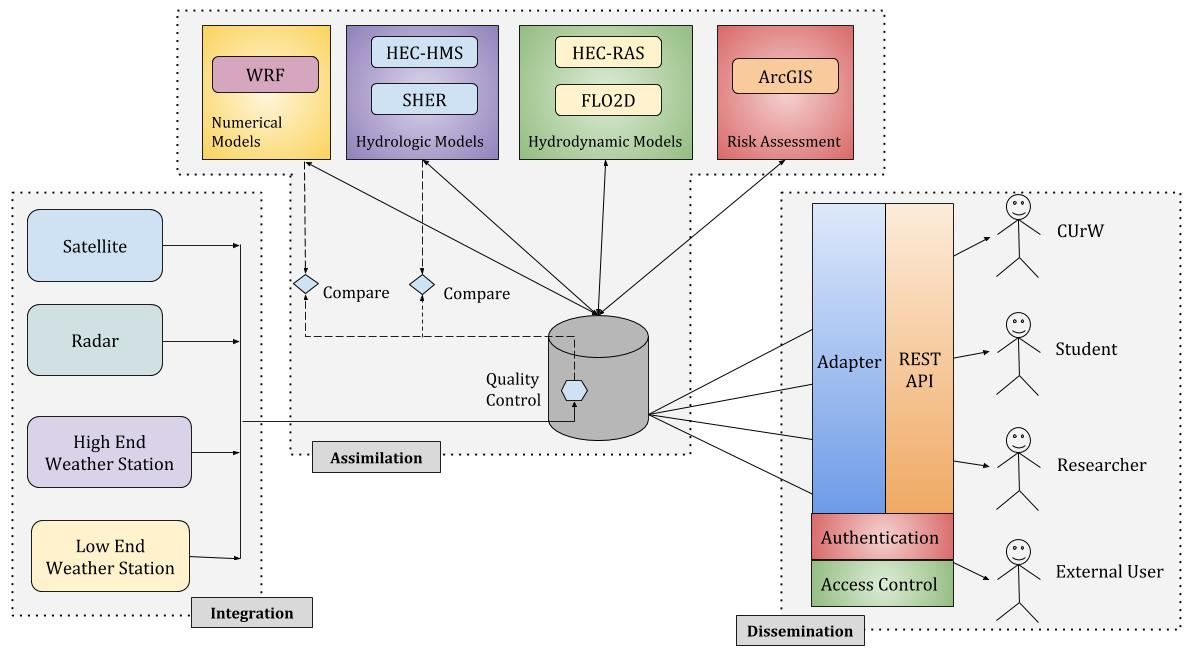
\includegraphics[width=0.5\textwidth]{method/misc/weather_data_system_components.jpg}}
\caption{Components of a weather data system.}
\label{pfi:wdia_components}
\end{figure}

The system should capable of integrating data from different source such as satellite data, high end and low end weather station etc in the form of multidimensional spatial and temporal weather data as shown in the \emph{Integration} modules.
Then the system should be able to fulfill weather models varying data requirements and should be able to store large set of redundant model data during the \emph{Assimilation} module.
The users should be able to easy to search into the available that in the system base on timeseries metadata or based on Geo queries, and the \emph{Dissemination} module should be capable of sharing data among different users.

The \acrshort{wdias} is supporting all three modules shown in \cref{pfi:wdia_components}. Through out the design phase of \acrshort{wdias}, we iterate through few architectures with concerning about the scalability and high availability. Initially, we followed \acrfull{soa} with using \acrfull{esb} to integrate different modules. However, we understood that \acrshort{esb} is not suitable for data streaming or bulk data processing and suffers from a single point of failure since it uses a common bus.
In second design phase, we used the Actor model with AKKA framework with following the microservice architecture such that each microservice is implemented using actors. Microservice architecture is resilient and flexible as one service is independent of another service enables to highly scalable individual services. One of the attractive features of microservice architecture is the independent nature of the microservices which allows to choose different technologies and maintain separately. But using AKKA framework for implement microservice architecture has some disadvantages such as unable to choose independent technologies and the actors messaging between different services cause to result in a too-tight code coupling between the services.

To overcome the issues using AKKA, we moved to the concept of container orchestration based microservice architecture. The \acrshort{wdias} used \acrfull{k8s} as the container orchestration system which is an open-source tool for automating deployment, scaling, and management of containerized applications. Using \acrshort{k8s}, users can add required resources as Nodes to the cluster, and K8s manage and deploy applications as pods into cluster nodes.
In next \cref{pse:wdias_architecture}, we discussed about the \acrshort{wdias} used microservice concepts such as implement microservice as dumb pipes rather implementing smart endpoints, uses database per service with access via API only, distributed Transactions over microservices using event processing, and considering distributed systems scalability in directions of x-axis scaling, y-axis scaling and z-axis scaling.

%%%%%%%%%%%%%%%%%%%%%%%%%%%%%%%%%%%%%%%%%%%%%%%%%%%%%%%%%%%%%%%%%%%%%%%%%%%%%%%%
\section{\db{Proposed Architecture}}
%\section{Weather Data Integration and Assimilation System Architecture}
\label{pse:wdias_architecture}

%%%%%%%%%%%%%%%%%%%%%%%%%%%%%%%%%%%%%%%%%%%%%%%%
\subsection{WDIAS Microservice Architecture}
\label{psubse:wdias_microservices}

\cref{pfi:microservice_separation} shows the clear separation of microservices into the modules of the \acrshort{wdias}. As seen in Figure of \cref{pfi:microservice_separation} and \cref{pfi:microservice_architecture_async} each circle represents a microservice in the \acrshort{wdias}, and those are implemented as containerized applications. 

\begin{figure}[htbp]
\centerline{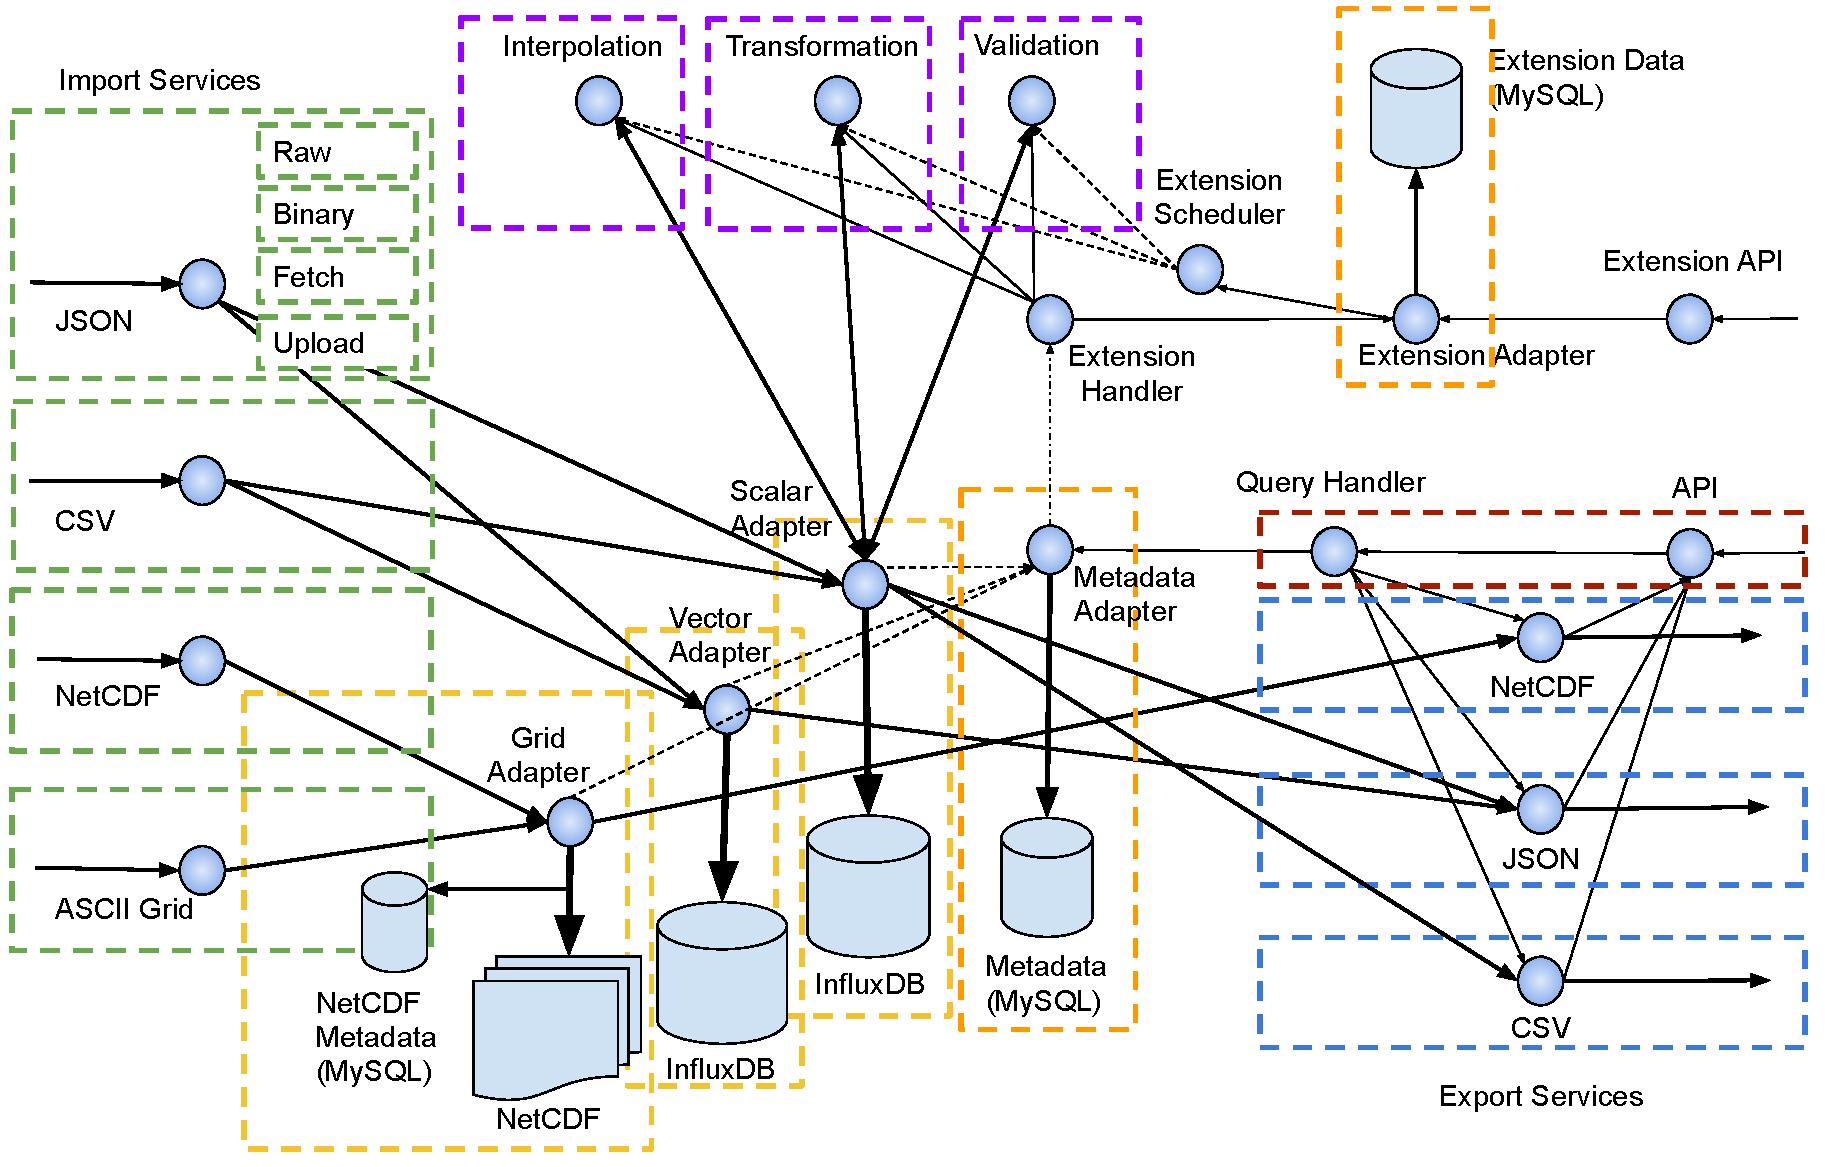
\includegraphics[width=0.5\textwidth]{method/microservice/separation_microservices-v4.pdf}}
\caption{Separation of \acrshort{wdias} microservices.}
\label{pfi:microservice_separation}
\end{figure}

\dbc{What tool did you used to generate these figures. If it support exporting images as PDF, use them with Latex as it gives you a vector image.}
\gkc{Replaced with PDF images.}

The left side of Figure 3.3 shows the import modules of the WDIAS, and the right side shows the export modules. each import microservice only does the specific task of converting and forwarding the request to the correct data adapter module. each data type, there is an adapter microservice is running which is optimized to storing such type of data. Each adapter has an isolated database, and the database is hosted separately for the high performance.
And timeseries metadata stored using RDBMS which gives more performance over retrieving metadata data, and cached with the in-memory database to fast access. The system generates a unique identifier for each timeseries, and throughout the WDIAS, other microservice use it to handle data for fast access. Export module microservice follows the same concepts and provides the capability to export the data into required formats of the weather models.

\begin{figure}[htbp]
\centerline{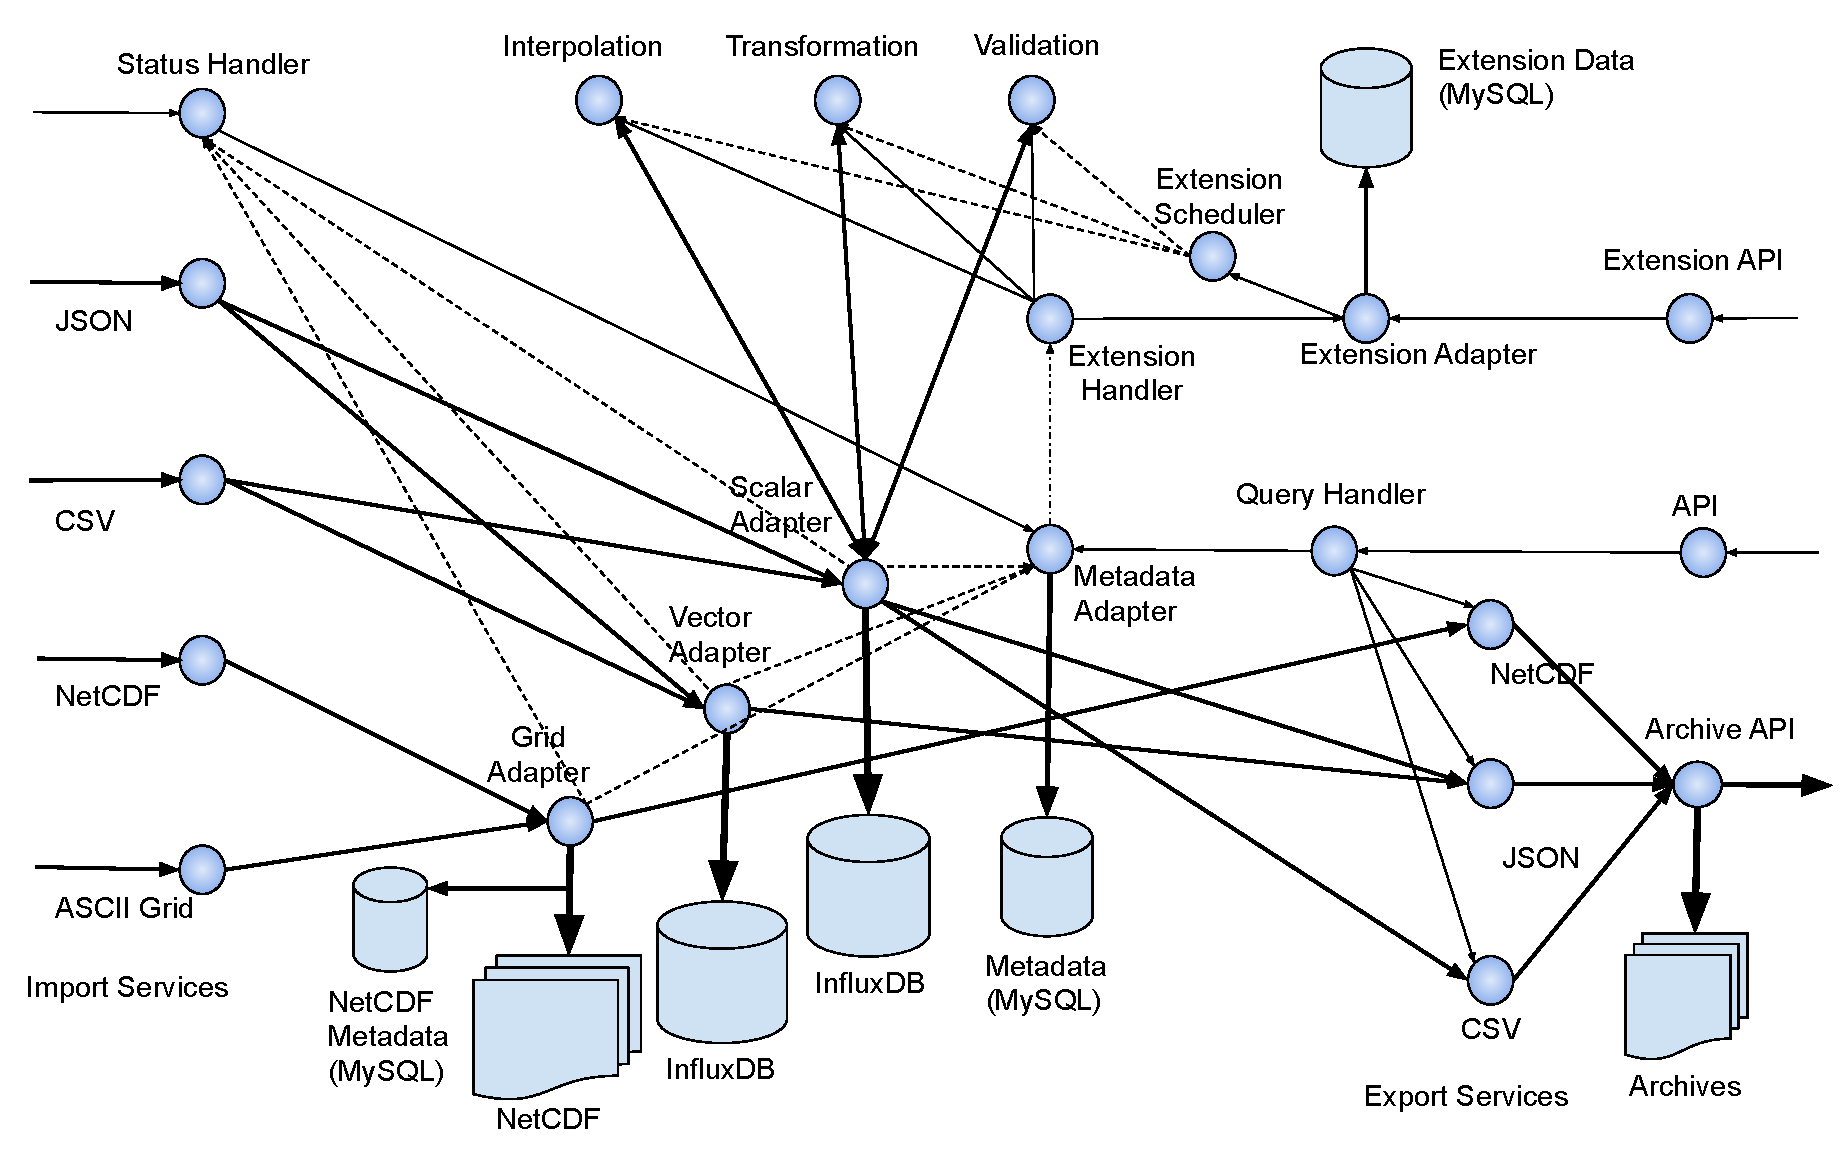
\includegraphics[width=0.5\textwidth]{method/microservice/microservice_architecture-handle_on_async-v4.pdf}}
\caption{microservice architecture - handle asynchronously.}
\label{pfi:microservice_architecture_async}
\end{figure}

As shown in Figure 3.4, when a request with a larger size comes to the system, it stores the data for asynchronously process the data and responds with a unique id that can use to verify whether data processed successfully or not. First it stores the data and publish an event to another service to process it. After successfully process the data by other service, it updates the system status. Also, the \acrshort{wdias} provides a simple RESTful API to interact with timeseries metadata and other modules such as import, export and extension modules.
\dbc{Drop the REST API. No need for a paper. You can briefly mention it.}
\gkc{Removed}

%%%%%%%%%%%%%%%%%%%%%%%%%%%%%%%%%%%%%%%%%%%%%%%%
\subsection{Database Structure}
\label{psubse:wdias_database}
\dbc{It's odd to start a sub-section after a very-long discussion. So add a sub-section for discussion up to this point.}
\gkc{Added a sub section above \cref{psubse:wdias_microservices}.}

The foundation of the \acrshort{wdias} is data-centric and build around the timeseries data.

\paragraph{Timeseries}-- \emph{A timeseries is simply a series of data points ordered in time}. In the weather domain, its interest in timeseries in perspective of observations to forecasting. Each timeseries, the data points can be formed in different formats as well. For example, scalar (0D), vector (1D), grid (2D), and polygon (2D).

Following list is the timeseries metadata which can use to uniquely identify one timeseries from another which are call as \emph{key attributes}.

\begin{itemize}
    \item \texttt{Module ID}--  String field which describe the source of the data generated.
    \item \texttt{Value Type}--  Scalar, Vector, Grid type
    \item \texttt{Location}-- Location of the timeseries. Point location, regular grid location or irregular grid location.
    \item \texttt{Parameter}-- variable measuring against a location
    \item \texttt{Timeseries Type} - Such as Historical or forecast
    \item \texttt{Time Step}-- Unit of Second, Minute, Hour, Day, Week, Month, Year, or NonEqualDistance. One of multiplier or divider can be used to define the interval between each measurement.
\end{itemize}

Scalar data point only consist of a single value. And Vector data point consists of two values such as magnitude and the direction of the Vector. But for Grid data, a point can consist of multiple values. To get the advantage of storing data efficiently, we can use a set of different databases based on the advantage of using them for each valueType. To support search queries with lower latency, it required to use indexing for the fast search for timeseries metadata. Further, Geo-based indexing is required to support Geo-based search queries based on the locations. Above capabilities achieved by using a database structure with compose of multiple databases as shown in \cref{pfi:database_structure}.

\begin{figure}[htbp]
\centerline{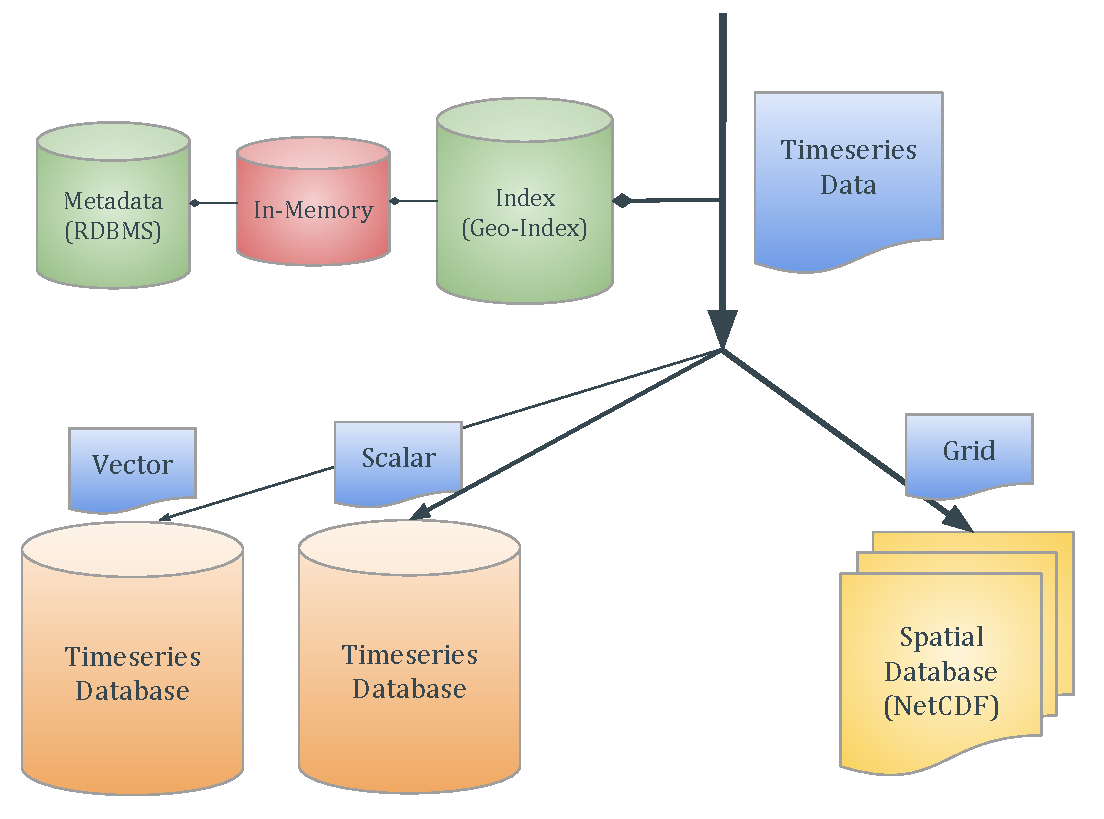
\includegraphics[width=0.4\textwidth]{method/microservice/wdias_database_structure.pdf}}
\caption{\acrshort{wdias} database structure.}
\label{pfi:database_structure}
\end{figure}

Since metadata consists of multiple key attributes, the data can be efficiently store using a Relational Database Management System (RDBMS). Two instances of Timeseries database is using in the WDIAS system by adapter-scalar and adapter-vector services. Use \acrfull{netCDF} for store the Grid data which support the creation, access, and sharing of array-oriented scientific data. And  in-memory database for caching for fast access the frequent access data in adapter-metadata and adapter-extension. Using a document-oriented database with support the Geo searching capabilities.

%%%%%%%%%%%%%%%%%%%%%%%%%%%%%%%%%%%%%%%%%%%%%%%%
\subsection{Weather Data Preprocessing}
\label{psubse:data_preprocessing}

The \acrshort{wdias} provides the data preprocessing capabilities via extension modules with a simple generic mathematical function model.

\begin{figure}[htbp]
\centerline{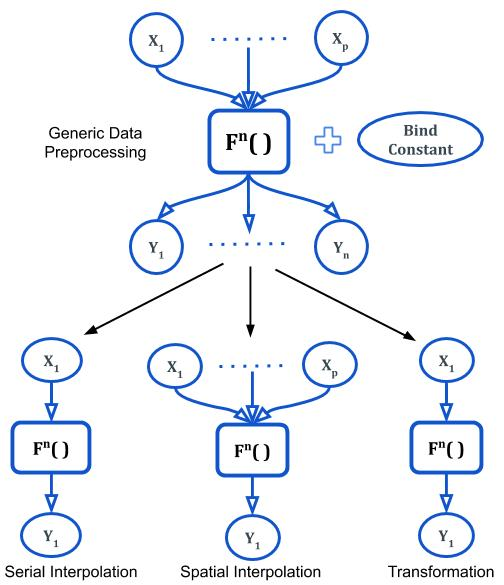
\includegraphics[width=0.4\textwidth]{method/data_preprocess/summary_weather_data_preprocessing.jpg}}
\caption{Generic functional approach to weather data preprocessing.}
\label{pfi:summary_weather_data_preprocessing}
\end{figure}

Each extension is considering as a mathematical function which can take \texttt{p} number of input timeseries variables and output \texttt{n} number of timeseries variables. Other than that, at the time of processing the system can configure to provide bind constant which can provide while configuring an extension. This means it is possible to change the behavior of an existing function by providing different bind constant at the time of creating new triggers for an extension. The system allow to create new triggers and update them at the run time via API with the POST request body shown in \cref{pli:extension_triggers}.

\begin{lstlisting}[language=Python, caption=Update Extension Triggers API, label=pli:extension_triggers]
{
    "extensionId": "", //Trigger unique identifier
    "extension": "Interpolation | Transformation | Validation",
    "function": "", //Mapping microservice
    "variables": [ //Timeseries mapping to variables
        {
            "variableId": "",
            "metadata/metadtaIds": {...}
        }
    ],
    "inputVariables": [], //Input timeseries
    "outputVariables": [], //Output timeseries
    "trigger": [ // When to trigger the function
        {
            "trigger_type": "OnChange | OnTime",
            "trigger_on": []
        }
    ],
    "options": { //Run time bind constant data
    }
}
\end{lstlisting}

\dbc{Code examples should be included only if they are novel and essential for discussion. If included, key lines in code need to be explained while referring to line numbers.}
\gkc{Updated.}

We implemented the system with possible to create multiple triggers for an extension such as Transformation can have two trigger to sample 1 minute data into 5 minutes data and 1 minute data into hourly data. Each extension trigger need to have a unique identifier as shown in Line 2. Then we allowed users to define the extension type (Line 3) and the microservice which is responsible of processing it (Line 4). User can map timeseries into variable and use them as \emph{X} input and \emph{Y} outputs in the \cref{pfi:summary_weather_data_preprocessing} (Line 5-12). Then provide when to trigger the extension with providing optional data as mentioned in the extension implementation.

\emph{Extension Handler} is responsible for triggering the correct Extension with metadata when there is any change on the subscribed extension trigger's \emph{OnChange} timeseries.
\emph{Extension Handler} is responsible for triggering the correct Extension with metadata at a given time which is provided at the creation on extension trigger with the value of \emph{OnTime} cronjob string value. To improve the performance of triggering cronjobs at given time schedules, the WDIAS added few optimization mechanisms.

%%%%%%%%%%%%%%%%%%%%%%%%%%%%%%%%%%%%%%%%%%%%%%%%
\subsection{Query Timeseries Metadata}
\label{psubse:query_timeseries}

Other than the metadata manipulation API mentioned in \cref{psubse:wdias_microservices}, the \acrshort{wdias} also supports timeseries search queries and Geo queries. As an example it can \emph{query timeseries available in a given area}. This operation uses \texttt{geoWithin} search operator for the simplicity. Other than it can also support query timeseries in an area by parameter, query available timeseries by locations and query locations within an area etc. In \cref{pli:geo_search}, the \acrshort{wdias} return the timeseries available within the area of a polygon provided as \emph{geoJson} \cite{InternetEngineeringTaskForceGeoJSON}.

\begin{lstlisting}[caption=Geo search timeseries, label=pli:geo_search]
    POST <HOST_NAME>/query/timeseries
    JSON Body:
    {
        "geoJson": {
            "type": "Polygon",
            "coordinates": [
                [
                    [<longitude>, <latitude>],
                    ...
                ]
            ]
        }
    }
\end{lstlisting}

%%%%%%%%%%%%%%%%%%%%%%%%%%%%%%%%%%%%%%%%%%%%%%%%%%%%%%%%%%%%%%%%%%%%%%%%%%%%%%%%
\section{Performance Analysis}
\label{pse:performance_analysis}

%%%%%%%%%%%%%%%%%%%%%%%%%%%%%%%%%%%%%%%%%%%%%%%%
\subsection{Load Testing Plan}
\label{psubse:test_plan}

The test plan is to perform load testing on whole system, and analyze the scalability of the system while measuring the operations perform on each module. Two variables can vary while doing performance testing.
\begin{enumerate}
    \item \acrfull{rps}
    \item Request size
\end{enumerate}

\acrshort{wdias} is getting a mix of all the data types in the percentages of 70\% scalar, 20\% vector, and 10\% grid values.
For a given request size the RPS increased in steps such as 600, 3000, 6000, 12000, and 18000 requests per minute. In each step, the RPS holds for a moment to give some time for the system to get stabilized after increasing linearly.

% \begin{figure}[htbp]
% \centerline{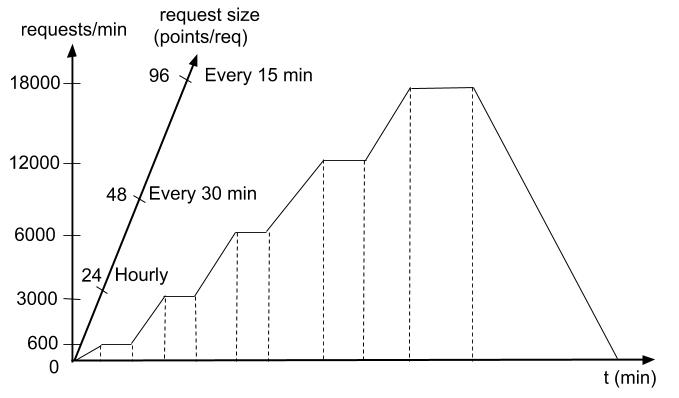
\includegraphics[width=0.5\textwidth]{results/work_load/performance_study_v4.jpg}}
% \caption{\acrshort{wdias} load testing plan with changing the request size and \acrshort{rps}}
% \label{pfi:performance_study}
% \end{figure}

\dbc{Drop pfi-performance-study figure. No need for paper. But explain key details in text.}
\gkc{Dropped the figure.}

Holding the peak load will help to show whether the system is capable of scaling more than the proposed load testing plan. After the peak, the test case goes through a cool-down period to measure the ability to shrink down the resources when there is not any load on the system. During the test plan, it runs for 30minutes of period with changing the request size form hourly data to 30 minutes data, then 15 minutes data. Then another 30 minutes load test enabling the auto scaling of container orchestration system, and perform 5minutes test run with timeseries queries. The the results are evaluate against the performance metrics of throughput, latency, resource utilization and auto-scaling.

%%%%%%%%%%%%%%%%%%%%%%%%%%%%%%%%%%%%%%%%%%%%%%%%
\subsection{Experimental Setup}
\label{psubse:experimental_setup}

During the performance test, it creates 1000 timeseries using the locations are taken from Google's Countries Public Data set \cite{GoogleGoogleCounties}, and uses static 100 Grid locations for store Grid data. Load test perform using  JMeter and used the Distributed Testing feature to generate higher load. It uses the master-slave approach and it allowed to handle all the test cases via single instance, rather handling separate instances. The system is capable of storing any numeric value up to 3 decimal points. It does not make any difference based on the parameter type whether it is the precipitation or the temperature. Thus, during the performance testing,  JMeter uses real precipitation data from \acrshort{curw}. One month period of data for five weather stations has been using to prepare the test data.

While implementing the test cases for WDIAS, it uses the Concurrency Thread Group
with Throughput Shaping Timer because it supports the open workload approach.

\begin{itemize}
    \item \emph{closed system model} \cite{Haggett1998AnWales} -- a new request is only triggered by the completion of a previous request, following by a think time.
    \item \emph{open system model} -- new requests arrival independently of completions.
\end{itemize}

\acrshort{wdias} is using the \acrfull{k8s} as the container orchestration system which is an open-source system for automating deployment, scaling, and management of containerized applications. They are many \acrshort{k8s} solutions available as a cloud service, we used \acrfull{eks} based on the availability. \cref{ptab:aws_eks_nodes} shows the list of nodes/computers used during the performance test.

\begin{table}[htbp]
\caption{\acrshort{eks} nodes}
\begin{center}
\begin{adjustbox}{width=0.45\textwidth}
\begin{tabular}{|l|r|r|r|r|l|}
\hline
\textbf{Node Label} & \textbf{vCPU} & \textbf{RAM (GB)} & \textbf{Storage (GB)} & \textbf{Quantity} & \textbf{EC2 Name} \\ \hline
core & 16 & 32 & 15 & 1 & c5.4xlarge \\ \hline
grid & 8 & 16 & 25 & 1 & c5.2xlarge \\ \hline
scalar & 8 & 16 & 20 & 1 & c5.2xlarge \\ \hline
test & 4 & 10.5 & 5 & 1 & c5n.xlarge \\ \hline
\end{tabular}
\end{adjustbox}
\label{ptab:aws_eks_nodes}
\end{center}
\end{table}

\dbc{All numerical values in tables must to right aligned.}
\gkc{Updated. Fixed the tables.}

To get better performance using the available resources, it is possible to schedule each microservice into a predefined set of nodes. Pods are assigned to the nodes \cref{ptab:aws_eks_nodes} based on the node label as below;
\begin{itemize}
    \item \emph{core} -- metadata, extensions, query, status and extension services
    \item \emph{grid} -- grid adapter, import and export grid data
    \item \emph{scalar} -- scalar and vector adapters, import and export of same data types
    \item \emph{test} --  JMeter and metric server
\end{itemize}

%%%%%%%%%%%%%%%%%%%%%%%%%%%%%%%%%%%%%%%%%%%%%%%%
\subsection{Performance Evaluation}
\label{psubse:performance_evaluation}

While performing the load testing, each test plan performed around 310k of total sample requests within 30minutes according to the \cref{ptab:obs_all_60_min_summary_throughput} to \cref{ptab:obs_all_15_min_summary_throughput}. The ratio between Scalar and Vector to Grid operations around 71k:8k with the ratio of 90\%:10\%. This implies that test cases were able to perform as planned in the \cref{psubse:test_plan}.
Other than insert Grid timeseries, other operations succeed with 0\% error rate.

\begin{table}[htbp]
\centering
\caption{Throughput and Latency of load testing with 60min data}
\begin{adjustbox}{width=0.45\textwidth}
% \footnotesize
\begin{tabular}{|l|r|r|r|r|r|r|}
\hline
\textbf{Label} & \textbf{Samples} & \textbf{Avg} & \textbf{90\%$^{\mathrm{a}}$} & \textbf{S.D.$^{\mathrm{b}}$} & \textbf{Error \%} & \textbf{RPS} \\ \hline
Insert Timeseries & 71826 & 28 & 31 & 58.74 & 0.00\% & 40.5 \\ \hline
Retrieve Timeseries & 71796 & 8 & 10 & 4.18 & 0.00\% & 40.7 \\ \hline
Insert Grid & 7982 & 23 & 26 & 4.23 & 0.06\% & 4.5 \\ \hline
Retrieve Grid & 7979 & 68 & 75 & 10.11 & 0.00\% & 4.5 \\ \hline
Query: Location & 71804 & 3 & 3 & 1.52 & 0.00\% & 40.5 \\ \hline
\textbf{TOTAL} & 311182 & 127 & 503 & 207.80 & 0.00\% & 175.4 \\ \hline
\multicolumn{4}{l}{$^{\mathrm{a}}$S.D.: Standard Deviation}{$^{\mathrm{b}}$90\%: 90\% percentile}
\end{tabular}
\end{adjustbox}
\label{ptab:obs_all_60_min_summary_throughput}
\end{table}

The average latency of inserting Scalar and Vector timeseries data increased by 1ms when the request size increased. But for the 90\% percentile of insertions increased from 31ms to 41ms. But the standard deviation kept same. \acrshort{wdias} were able to perform with the same throughput of 40.5 \acrshort{rps} without significant change in latency which shows the scalability of the system.
While retrieving the Scalar and Vector timeseries data, the system was able to respond with in 10ms for 60minutes and 30minutes data with lesser standard deviation. But the latency got double when handling the 15minutes data. This caused by heavy writes on the timeseries database.

\begin{table}[htbp]
\caption{ Throughput and Latency of load testing with 30min data}
\begin{center}
\begin{adjustbox}{width=0.45\textwidth}
% \footnotesize
\begin{tabular}{|l|r|r|r|r|r|r|}
\hline
\textbf{Label} & \textbf{Samples} & \textbf{Avg} & \textbf{90\%$^{\mathrm{a}}$} & \textbf{S.D.$^{\mathrm{b}}$} & \textbf{Error \%} & \textbf{RPS} \\ \hline
Insert Timeseries & 71759 & 29 & 32 & 50.97 & 0.00\% & 40.5 \\ \hline
Retrieve Timeseries & 71730 & 9 & 10 & 6.04 & 0.00\% & 40.6 \\ \hline
Insert Grid & 7972 & 44 & 49 & 8.17 & 0.08\% & 4.5 \\ \hline
Retrieve Grid & 7971 & 81 & 93 & 15.15 & 0.00\% & 4.5 \\ \hline
Query: Location & 71734 & 3 & 3 & 1.90 & 0.00\% & 40.5 \\ \hline
TOTAL & 310878 & 129 & 0 & 207.10 & 0.00\% & 175.3 \\ \hline
\multicolumn{4}{l}{$^{\mathrm{a}}$S.D.: Standard Deviation}{$^{\mathrm{b}}$90\%: 90\% percentile}
\end{tabular}
\end{adjustbox}
\label{ptab:obs_all_30_min_summary_throughput}
\end{center}
\end{table}

When inserting the Grid timeseries data, the average latency was less than the insert Scalar or Vector data, because of the Grid data handle asynchronously. When the number of Grid files doubled, each time the latency also got doubled. Notably, the \acrshort{wdias} was able to perform with same throughput with lesser standard deviation. Also, for each test case the system was able to kept the same latency throughout test run without any significant change. This also show the scalability of the Grid data in the \acrshort{wdias}.
Retrieving of Grid timeseries data happens on demand during the load test. But it is possible to upgrade the system to support asynchronously download alongside with direct download. Because of that, the latency of download the the Grid data is bit higher than the other test cases. In that case also, the \acrshort{wdias} perform with keeping the same throughput with lower standard deviation which shows the scalability of the export Grid data module.

\begin{table}[htbp]
\caption{ Throughput and Latency of load testing with 15min data}
\begin{center}
\begin{adjustbox}{width=0.45\textwidth}
% \footnotesize
\begin{tabular}{|l|r|r|r|r|r|r|}
\hline
\textbf{Label} & \textbf{Samples} & \textbf{Avg} & \textbf{90\%$^{\mathrm{a}}$} & \textbf{S.D.$^{\mathrm{b}}$} & \textbf{Error \%} & \textbf{RPS} \\ \hline
Insert Timeseries & 71775 & 30 & 41 & 51.71 & 0.00\% & 40.5 \\ \hline
Retrieve Timeseries & 71736 & 23 & 32 & 50.18 & 0.00\% & 40.6 \\ \hline
Insert Grid & 7975 & 91 & 112 & 19.58 & 1.42\% & 4.5 \\ \hline
Retrieve Grid & 7972 & 118 & 165 & 56.15 & 0.00\% & 4.5 \\ \hline
Query: Location & 71749 & 3 & 4 & 2.32 & 0.00\% & 40.5 \\ \hline
\textbf{TOTAL} & 310934 & 134 & 503 & 206.40 & 0.04\% & 175.4 \\ \hline
\multicolumn{4}{l}{$^{\mathrm{a}}$S.D.: Standard Deviation}{$^{\mathrm{b}}$90\%: 90\% percentile}
\end{tabular}
\end{adjustbox}
\label{ptab:obs_all_15_min_summary_throughput}
\end{center}
\end{table}

Throughout all test plans, the \acrshort{wdias} system performed better on serving the search queries based locations for Scalar and Vector timeseries. This is due to using indexing for server such queries. The \acrshort{wdias} was able to respond with 3ms most of the cases with keeping lower standard deviation.
% To get better performance test on the query module, we performed set of complex queries as shown in the \cref{ptab}

\begin{table}[htbp]
\caption{Throughput and Latency of load testing with 15min data while enabled K8s auto-scaling}
\begin{center}
\begin{adjustbox}{width=0.45\textwidth}
\footnotesize
\begin{tabular}{|l|r|r|r|r|r|r|}
\hline
\textbf{Label} & \textbf{Samples} & \textbf{Avg} & \textbf{90\%$^{\mathrm{a}}$} & \textbf{S.D.$^{\mathrm{b}}$} & \textbf{Error \%} & \textbf{RPS} \\ \hline
Insert Timeseries & 71727 & 34 & 27 & 118.78 & 0.00\% & 40.5 \\ \hline
Retrieve Timeseries & 71693 & 7 & 9 & 18.72 & 0.00\% & 40.5 \\ \hline
Insert Grid & 7968 & 87 & 98 & 14.07 & 0.18\% & 4.5 \\ \hline
Retrieve Grid & 7965 & 89 & 110 & 37.79 & 0.00\% & 4.5 \\ \hline
Query: Location & 71704 & 1 & 2 & 2.05 & 0.00\% & 40.5 \\ \hline
\textbf{TOTAL} & 310734 & 130 & 501 & 212.35 & 0.00\% & 175.3 \\ \hline
\multicolumn{4}{l}{$^{\mathrm{a}}$S.D.: Standard Deviation}{$^{\mathrm{b}}$90\%: 90\% percentile}
\end{tabular}
\end{adjustbox}
\label{ptab:obs_all_auto_15_min_summary_throughput}
\end{center}
\end{table}

\cref{ptab:obs_all_auto_15_min_summary_throughput} shows the \acrshort{wdias} performance with 15minutes data, but enabled auto-scaling. During above test cases, most resource utilized module was importing Grid data.
The observations are almost similar to \cref{ptab:obs_all_15_min_summary_throughput}, but notably the error rate of insert Grid timeseries got reduced after enabled the auto-scaling for import Grid data module. Also, the standard deviation for handling Grid data reduced which means system was able to perform more better than the previous test plan.

\begin{figure}[htbp]
\centerline{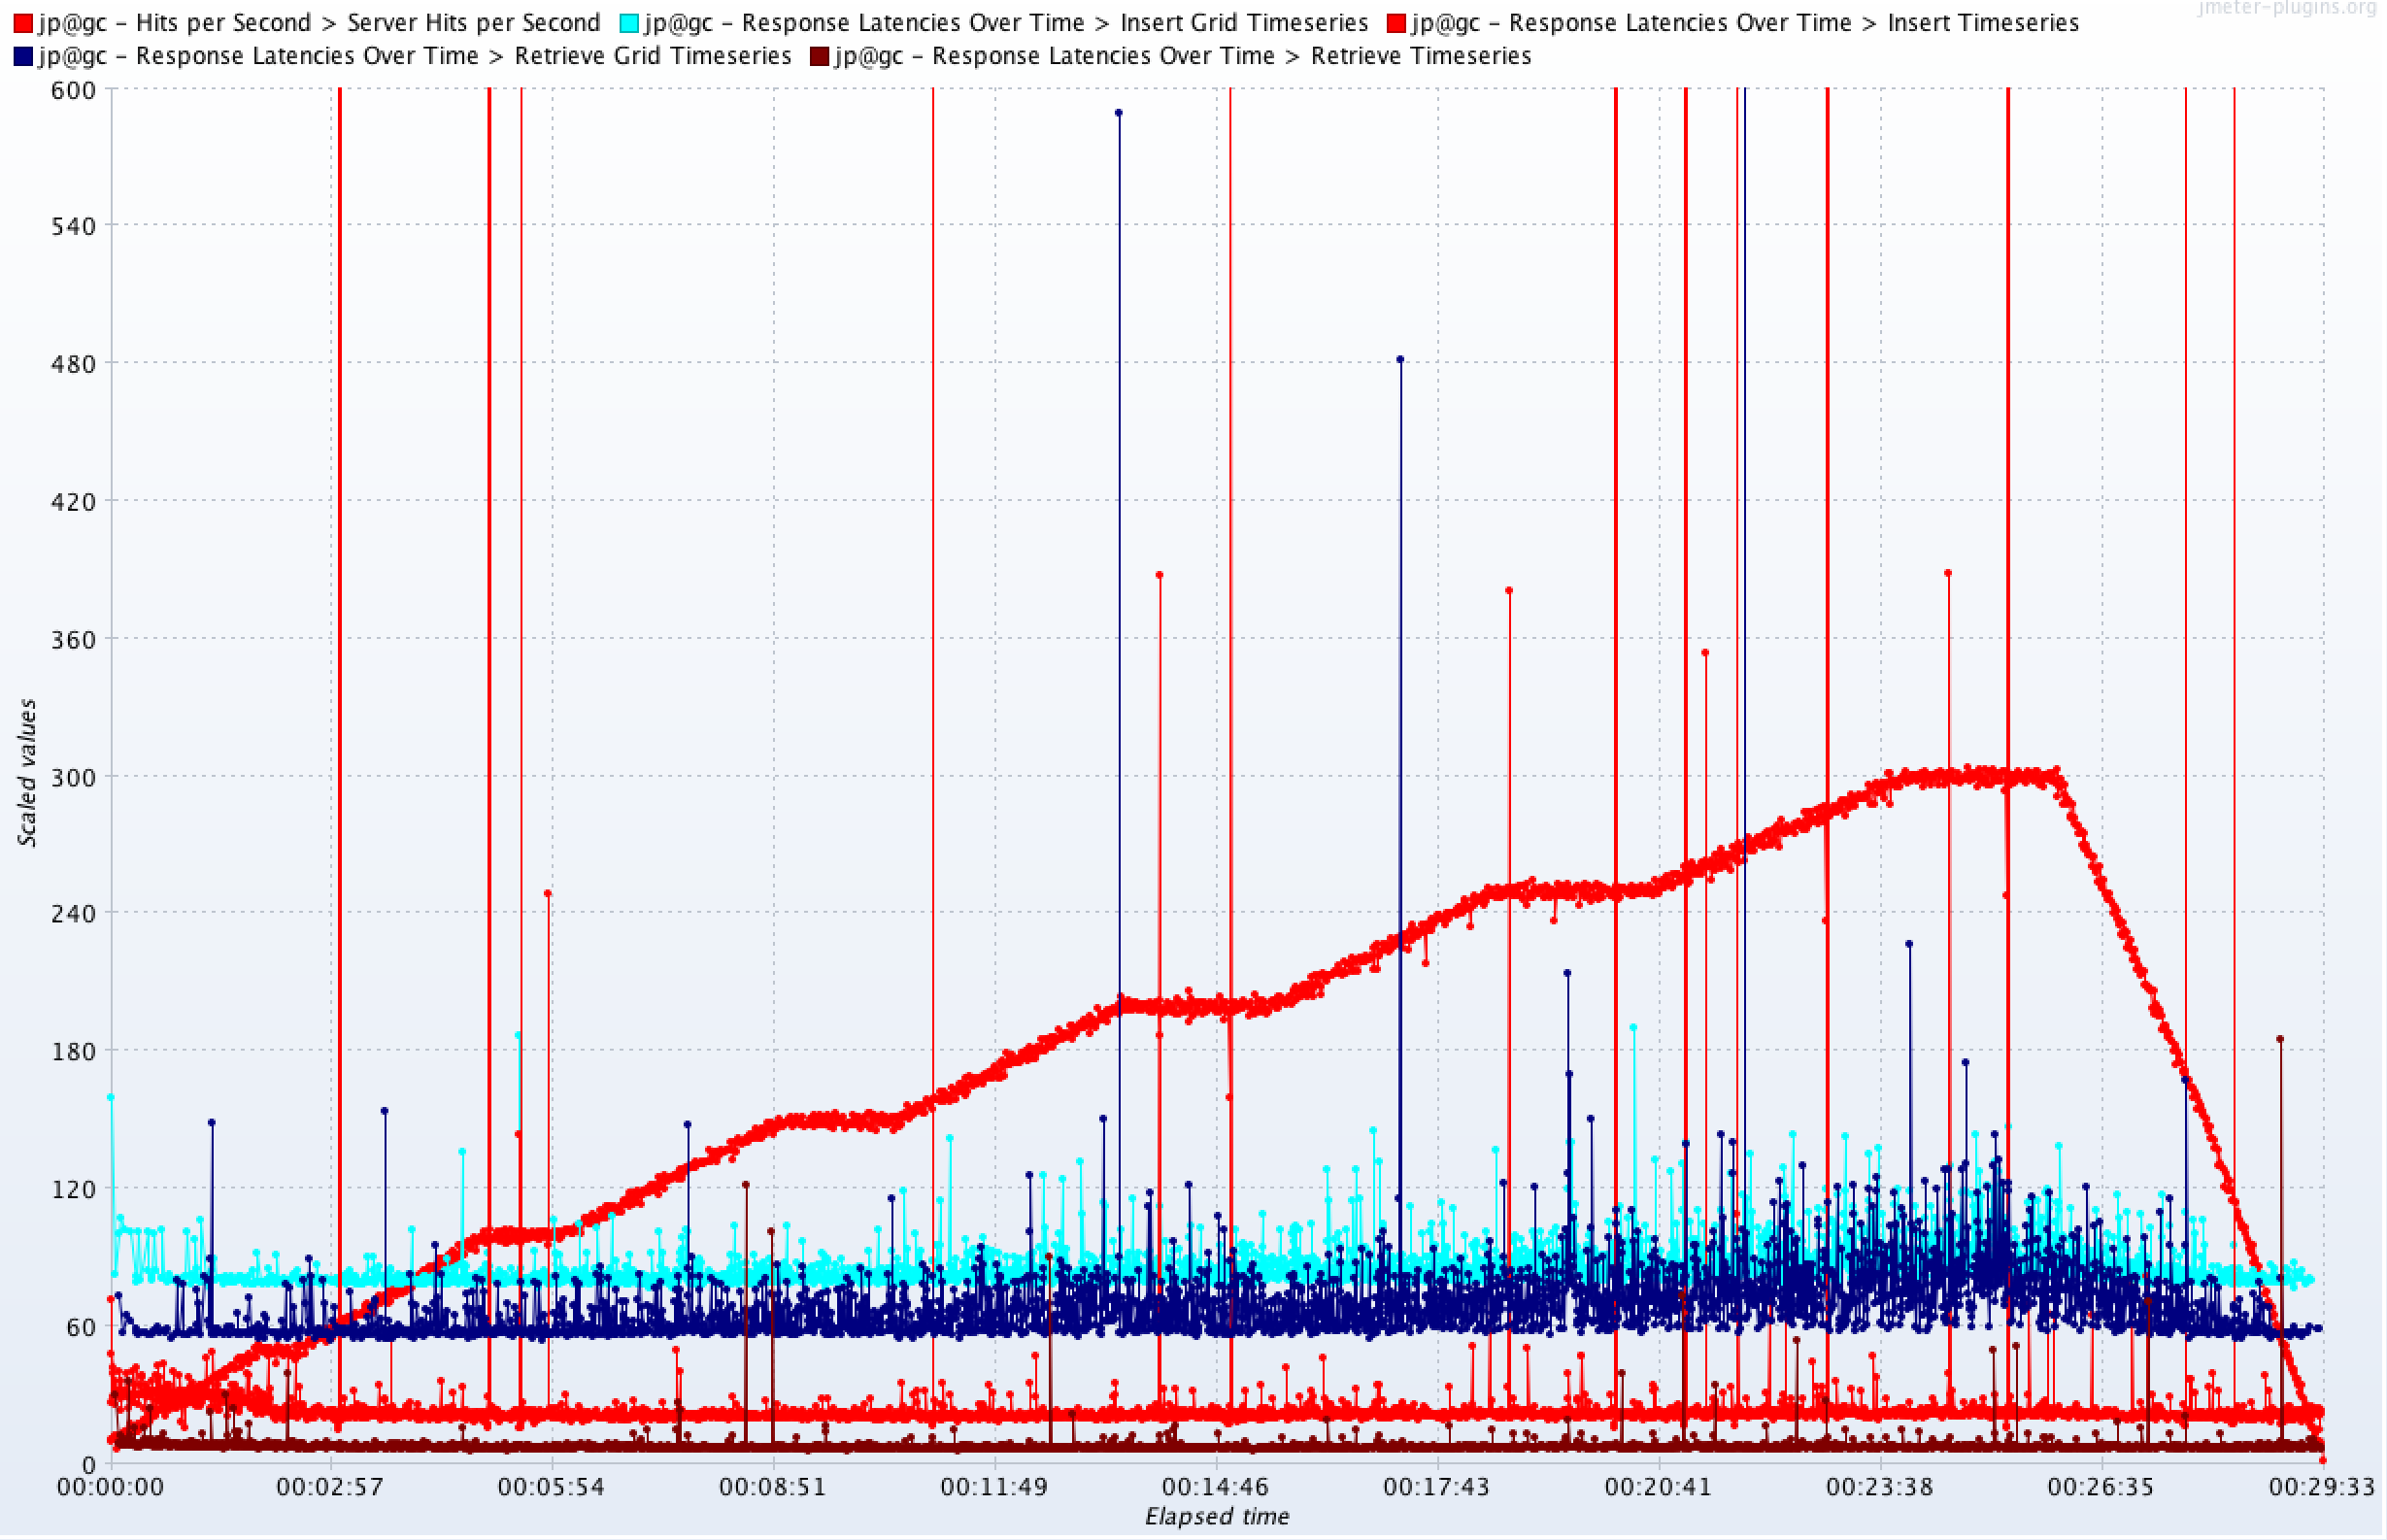
\includegraphics[width=0.5\textwidth]{results/obs/all_auto/obs_all_auto_15m_res_latencies_against_hits.png}}
\caption{Performance test 15min data enabled auto-scaling - response latencies against server hits over the elapsed time.}
\label{pfi:test_obs_auto_all_15_min_latency_vs_hits}
\end{figure}

\cref{pfi:test_obs_auto_all_15_min_latency_vs_hits} shows the latency of each test case throughout total time of load testing with 15minutes data while enabled auto-scaling. As the Figure clearly shows while increasing the number of server hits for each test case, the system kept the latency constant without significant change. At the peak time, handling Grid data has some disturbances and inserting Scalar and Vector data has some random spikes in the latencies.

\begin{figure}[htbp]
\centerline{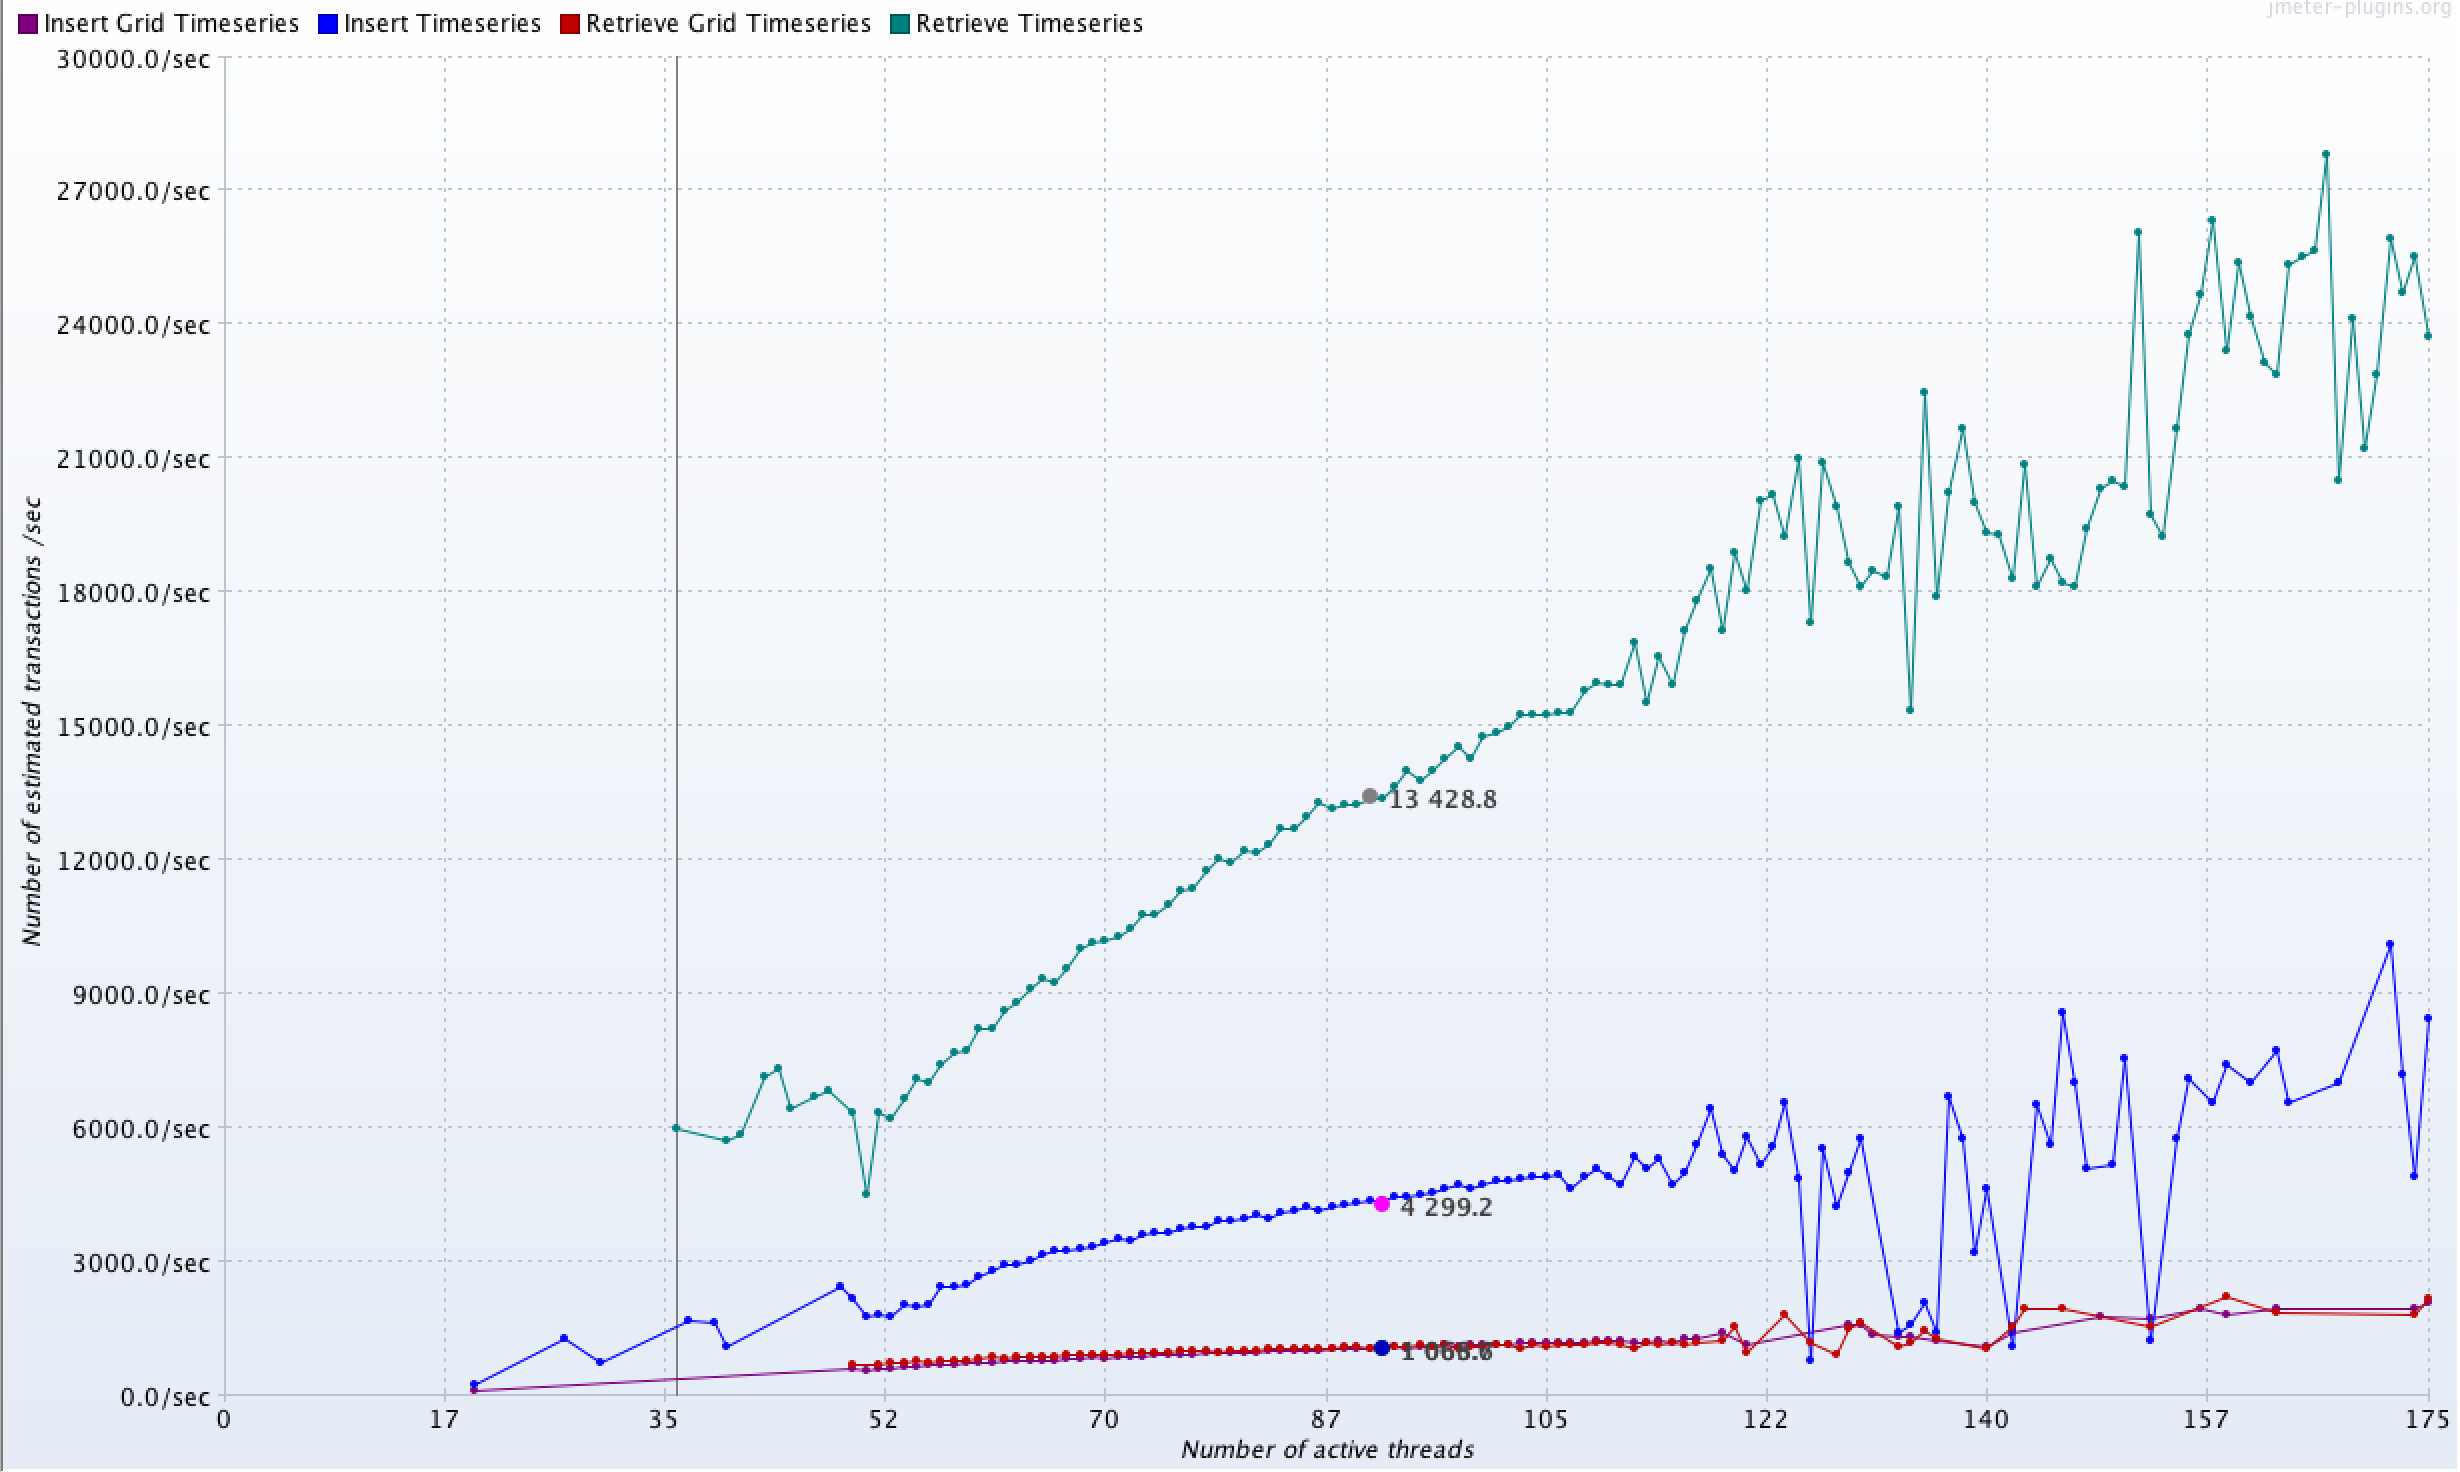
\includegraphics[width=0.5\textwidth]{results/obs/all_auto/obs_all_auto_15m_transaction_throughtput_vs_threads.png}}
\caption{Performance test 15min data enabled auto-scaling - transnational throughput vs number of active threads.}
\label{pfi:test_obs_auto_all_15_min_throughput_vs_threads}
\end{figure}

\cref{pfi:test_obs_auto_all_15_min_throughput_vs_threads} shows the total server's transaction throughput against the number of active threads.
The formula for total server transaction throughput is \(<active threads> * 1 second / <1  thread response time>\) \cite{JMeterPluginsTransactionPlugin}. It shows the statistical maximum possible number of transactions based on the number of users accessing the application.
By combining the \cref{pfi:test_obs_auto_all_15_min_latency_vs_hits}, this graph shows that the throughput of the system gets increased without much change in the latency, thus it proves the scalability of the \acrshort{wdias}.

\begin{figure}[htp]
    \centering
    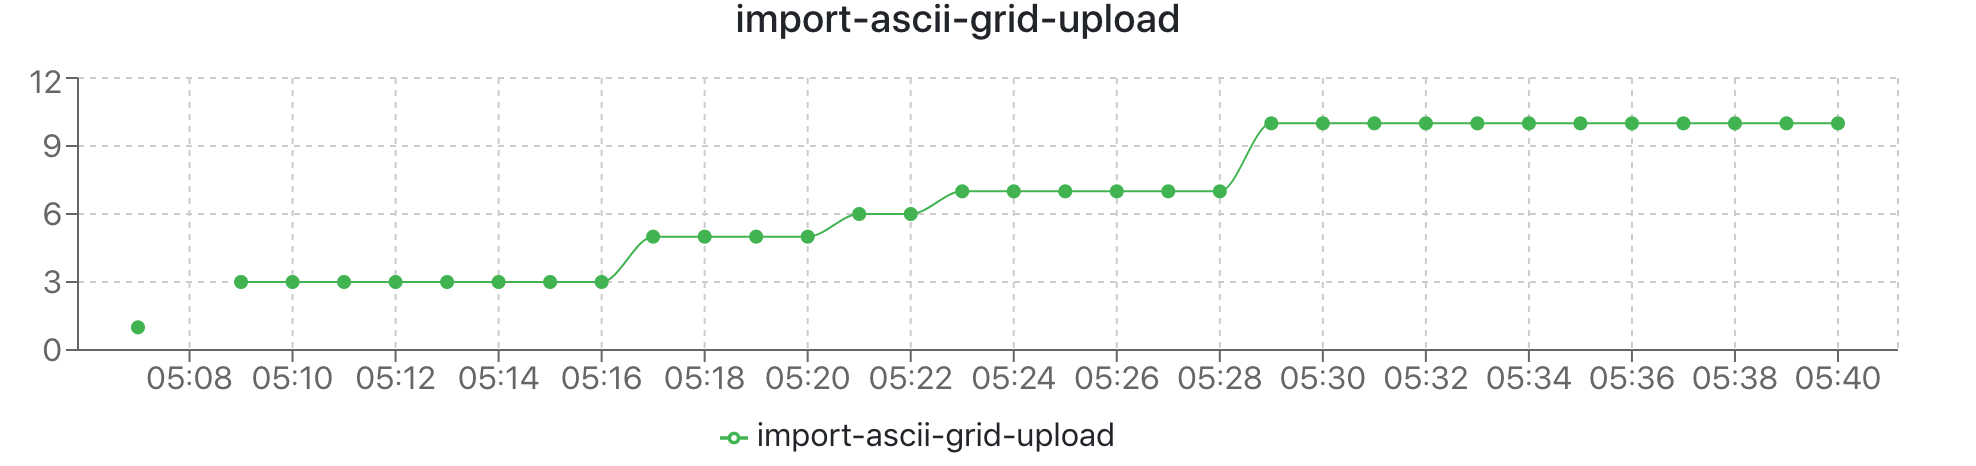
\includegraphics[width=0.5\textwidth]{results/obs/all_auto/obs_all_auto_15m_import_grid_pod.png}
    \caption{Load testing with auto-scaling import ascii grid number of pods over time.}
    \label{pfi:obs_all_auto_15m_import_grid_pod}
\end{figure}

\cref{pfi:obs_all_auto_15m_import_grid_pod} shows the number of import-ascii-grid-upload pods scheduled overtime. The auto-scaling enabled with the configurations of 1 to 10 pods with the recommended CPU usage with 80\%. And the pods scheduled with 1 CPU requested, and limit with 2 CPUs per pod.
As the graph shows, 3 pods scheduled at the initial as per the configuration of the helm chart. While increasing the workload, new pods get spawn while keeping the constraint of 80\% of recommended CPU utilization. After \acrshort{k8s} spawn 10 maximum pods, it stops spawning new pods. But the pods were able to perform with vertical scaling since those are not hit the CPU limit of 2.

%%%%%%%%%%%%%%%%%%%%%%%%%%%%%%%%%%%%%%%%%%%%%%%%
\subsection{Performance Metrics Analysis}
\label{psubse:performance_metrics}

The \emph{Latency} for each operation type kept constant over the whole test plan run time without any significant change. When the request size increased from 24 data points to 96 data points, the latency increase throughout the whole test plan with a smaller number. But for each test run, the latency kept constant over time.
During the \cref{ptab:obs_all_auto_15_min_summary_throughput} test run, the performance of the Grid data got better when compared to \cref{ptab:obs_all_15_min_summary_throughput}. This means by adding more resources to the \acrshort{wdias}, it can handle more workload on the system.

While keeping the latency constant without significant change, the \emph{throughput} of the \acrshort{wdias} kept constant while increasing the request size from 60min data (24 data points) to 15min data (96 data points) for all the data types such as Scalar, Vector, and Grid.
When the number of active threads increased, the \acrshort{wdias} able to provide the same throughput with maintaining the latency stable.

One of the reasons for having deviations at the peak time due to uses of single instance for the data consistency such as  InfluxDB for Scalar and Vector data, and netCDF with parallel support for Grid data. Further, it is possible to gain more performance using the databases with configure with high scalability and high availability features such as Sharding and Replication.

When looking into the \emph{resource utilization} of \acrshort{wdias}; since it is using the \acrshort{k8s} as the container orchestration system, it allows us to scale up and cool down the system as required based on the workload. This demonstrates the test plan of \cref{ptab:obs_all_15_min_summary_throughput}, and the system gets scale up to the maximum at the peak time. Then cool down to a single pod after finishing the test cases.
Given above \acrshort{wdias} can run from 1 CPU node to nodes with 100 CPUs. As described in the \cref{pse:wdias_architecture}, it uses many of the concepts of modern microservice architecture to create stateless, failover, redundant microservice to achieve such capabilities.

The \acrshort{wdias} supports \emph{auto scaling} by out of the box with \acrshort{k8s}. Services can configure with a maximum number of pods to avoid over resource usage. When there is not much workload on the system, the system cools down to fewer pods to save more resources. When there is an issue with a pod, \acrshort{k8s} auto-schedule another pod and remove the unhealthy pod. Also, it allows updating the system without any downtime with rollback updates.

\emph{Risk of unable to process data} during the test performance, the \acrshort{wdias} processed many requests with higher request size than the normal usage with a lower rate of failures to process the requests, mainly with insert Grid data. If the usage of \acrshort{wdias} wants to reduce the risk of unable to process data, then the system can configure to run with redundant pods to handle spike of workloads. Also, while configuring for the auto-scaling, the \acrshort{k8s} can configure to maintain a lower amount of CPU usage such as 50\% to 60\% rather  than 80\%. Such configuration with always spawn new pods to handle double of current peak load.

%%%%%%%%%%%%%%%%%%%%%%%%%%%%%%%%%%%%%%%%%%%%%%%%%%%%%%%%%%%%%%%%%%%%%%%%%%%%%%%%
\subsection{Discussion}
\label{psubse:discussion}
\dbc{Make this the discussion and a sub-section of Sec. 4}
\gkc{Renamed. I did not get what did you mean by sub Section 4. Did you mean \cref{pse:summary}?}

As we showed that the \acrshort{wdias} can perform better, there are some improvements that can add to improve the performance and usability of the system.

\emph{Lack of data preprocessing modules}:
The extension module enables the plugin system to integrate prepossessing modules that can use for process the data which are inserted to the system or based on regular intervals. Also, \acrshort{wdias} provides a more generic open interface approach to create more preprocessing modules. Since \acrshort{wdias} is an open-source system, it expects more modules to be created by the community. When compared to other systems like \acrshort{fews}, the current system only have few extensions but it is more easy to add new extensions compared to other systems.

Improve the \emph{Grid data performance} by porting \acrshort{netCDF} C or FORTRAN implementation with adapter-grid rather using a Python wrapper. Using tools like Terraform which is independent of the Cloud Computing provider \emph{define \acrshort{wdias} infrastructure as code}, then users will able to easily deploy the \acrshort{wdias} on any Cloud provider without much hassle. \emph{Tune \acrshort{wdias} database structure performance} with using z-axis scaling. Some of other features are alerting extension modules, publisher subscriber capabilities via extension modules, supporting irregular Grids.

%%%%%%%%%%%%%%%%%%%%%%%%%%%%%%%%%%%%%%%%%%%%%%%%%%%%%%%%%%%%%%%%%%%%%%%%%%%%%%%%
\section{Summary}
\label{pse:summary}
\dbc{Summary is too long. Should not be more than a single para}
\gkc{Just kept the important sections}
\dbc{Summary should not be more than a single para for a paper.}
\gkc{Reduce to one paragraph with removing some info.}

In this paper, we present an extendable open source weather data integration and assimilation system to overcome the issues in existing systems. Most systems are proprietary or closed source, based on client-server architectures or monolithic distributed system architectures, and depend on computer platforms unable to use could computing to gain benefits of scalability, high availability and low-cost operations. The proposed system uses modern microservice architecture pattern and cloud computing tools such as container orchestration to gain high scalability and availability. Based on the nature of the weather metadata, the \acrshort{wdias} used a database structure to provide higher performance while storing the weather data optimum. \acrshort{wdias} uses many microservice architecture concepts to create stateless, failover, and redundant microservice with providing a generic open mechanism to integrate new modules as an extension to enhance the features of the system and weather data preprocessing. Further, the system provides an extension API to easy access to create and modify the extension triggers on the fly and support complex timeseries metadata queries with Geo-based support.
We used an experimental \acrshort{k8s} setup on Cloud infrastructure for the performance analysis, and the \acrshort{wdias} able to handle 18,000 requests per minute successfully with minimizing the error rate to zero. Also, we repeated the test cases while increasing the request size. The system handled increasing workload same while keeping the latency constant without any significant change and able increase the throughput. With referring to above facts, it shows the scalability of the \acrshort{wdias} system.
Using \acrshort{k8s} auto-scaling, the system were able to elastically adjust the number of pods to handle the workload and shows that the system can run from few CPU node to nodes with a few hundred CPUs.

%%%%%%%%%%%%%%%%%%%%%%%%%%%%%%%%%%%%%%%%%%%%%%%%%%%%%%%%%%%%%%%%%%%%%%%%%%%%%%%%
\section*{Acknowledgment}
\label{pse:ack}
This research is supported in part by the grant from the Center for Urban Water, Sri Lanka.

%%%%%%%%%%%%%%%%%%%%%%%%%%%%%%%%%%%%%%%%%%%%%%%%%%%%%%%%%%%%%%%%%%%%%%%%%
\graphicspath{ {./images/} }
\newacronym{wdias}{WDIAS}{Weather Data Integration and Assimilation System}

\newacronym{fews}{Delft-FEWS} {Delft-FEWS, Deltares}
\newacronym{lead}{LEAD}{Linked Environments for Atmospheric Discovery}
\newacronym{dias}{DIAS}{Data Integration and Assimilation System}
\newacronym{madis}{MADIS}{Meteorological Assimilation Data Ingest System}

\newacronym{nwm}{NWMs}{Numerical Weather Models}
\newacronym{NetCDF}{NetCDF}{Network Common Data Form}
\newacronym{soa}{SOA}{Service Oriented Architecture}
\newacronym{wrf}{WRf}{Weather Research and Forecast}
\newacronym{esb}{ESB}{Enterprise Service Bus}
\newacronym{microservice}{Microservice}{Microservice Architectire}

\newacronym{curw}{CUrW SL}{Urban Center for Water, Sri Lanka}
\printbibliography[title={References}]
\dbc{References must be in IEEE standard. Some are not quite formatted for IEEE standard. For e.g., some of the paper and conference titles are in upper case.}
\gkc{I got your point. But I used this IEEE template: https://www.overleaf.com/latex/templates/ieee-conference-template-example/nsncsyjfmpxy. Not sure how to fix it. May be need to edit the Class implementation above.}
\gkc{Updated. Mendeley has imported them in Upper case. Still is there any issue?}

\end{document}
